\section{Wartości bezwzględne na ciele}
Tu $\R_+ = \{x \in \R : x \ge 0\}$, zaś $\cialo$ jest ciałem.

\begin{definicja}
	\emph{Wartość bezwzględna} to funkcja $\|\cdot\| \colon \cialo \to \R_+$, że $\|x\| = 0$ tylko dla $x = 0$, dla wszystkich $x, y \in \cialo $ zachodzi $\|xy\| = \|x\| \cdot \|y\|$ oraz $\|x + y\| \le \|x\| + \|y\|$.
	Jeśli jest jeszcze $\|x+y\| \le \max \{\|x\|, \|y\|\}$, to jest \emph{niearchimedesowa}.
\end{definicja}

\begin{fakt}
	Na skończonym ciele istnieje tylko trywialna norma.
\end{fakt}

\begin{proof}
	Wynika to z twierdzenia Lagrange'a dla $\cialo^\times$.
\end{proof}

\begin{definicja}
	Funkcja $v_p \colon \Z \setminus \{0\} \to \R$, ,,największy wykładnik $v$, że $p^v$ dzieli argument'', to waluacja $p$-adyczna.
\end{definicja}

Przedłuża się do ciała $\Q$: $v_p(x/y) = v_p(x) - v_p(y)$, $v_p(0)$ to ,,$\infty$''.
Jest dobrze określona.
Ogólniej przez waluację rozumie się każdą funkcję, dla której prawdziwy jest poniższy lemat.

\begin{lemat}
	Niech $x, y \in \Q$.
	Wtedy $v_p(xy) = v_p(x) + v_p(y)$ i $v_p(x+y) \ge \min \{v_p(x), v_p(y)\}$ z umową dla $v_p(0)$.
\end{lemat}

Waluacja i wartość bezwzględna mają podobne własności: produkt zamienił się w sumę (logarytm), sama zaś nierówność odwróciła się.
Potęgowanie i ponowne odwrócenie dowodzą:

\begin{fakt}
	Funkcja $|x|_p = p^{-v_p(x)}$ to niearchimedesowa norma.
\end{fakt}

\begin{fakt}
	Jeśli $\pierscien$ jest dziedziną całkowitości z ciałem ułamków $\cialo$, zaś $v \colon \pierscien \setminus \{0\} \to \R$ waluacją przedłużoną do całego $\cialo$ wzorem $v(x/y) = v(x)-v(y)$, to funkcja $\cialo \to \R_+$, $\|z\|_v = \exp(-v(z))$ i $\|0\| = 0$ jest niearchimedesową wartością bezwzględną.
	Odwrotnie, gdy $\|\cdot\|$ nią jest, to $-\log \|\cdot\|$ jest waluacją.
\end{fakt}

\begin{fakt}
	Norma $\|\cdot\|$ na ciele $\cialo$ jest niearchimedesowa, wtedy i tylko wtedy, gdy $\|n\| \le 1$ dla każdego $n \in \Z$ (włożonego w $\cialo$).
\end{fakt}

\begin{proof}
	Implikacja w jedną stronę jest oczywista, bo przecież $\|\pm 1\| = 1$ pociąga $\|n \pm 1\| \le \max \{\|n\|, 1\}$ i indukcja kończy dowód.
	W lewą stronę wymagane są już czary-mary.
	Ponieważ $\|x + y\| \le \max \{\|x\|, \|y\|\}$ jest oczywista dla $y = 0$, wystarczy dowieść $\|z+1\| \le \max \{\|z\|, 1\}$ ($z \in \cialo$).
	Dla $n \in \N$:
	\begin{align*}
		\|z+1\|^m & = \left\|\sum_{i=0}^m {m \choose i} z^i \right\| \le \sum_{i=0}^m \left\|{m \choose i} z^i \right\| \le \sum_{i=0}^m \|z\|^i \\
		& \le (m+1) \max \{1, \|z\|^m\}
	\end{align*}
	Przechodzimy z $m$ do $+ \infty$ po spierwiastkowaniu.
\end{proof}

Własność Archimedesa mówi, że $\sup\{|n| : n \in \Z\} = \infty$.
Jeżeli supremum jest skończone, to wynosi $1$ i wartość nie jest archimedesowa.

\begin{historia}[Archimedes z Syrakuz]\end{historia}

\section{Fałszywa geometria}
Ciało, gdzie wszystkie działania są ciągłe, nazywa się ciałem topologicznym, takie może być ciało z metryką.

Przestrzenie z taką nierównością wydają się być dziwaczne i rzeczywiście nimi są.
Skoro pomiar odległości nie należy do normalnych, to i geometria będzie nie z tej Ziemi.

\begin{fakt}
	W niearchimedesowym ciele $\cialo$, $\|x\| \neq \|y\|$ pociąga $\|x+y\| = \max \{\|x\|, \|y\|\}$.
\end{fakt}

\begin{proof}
	$\|x\| > \|y\|$ pociąga $\|x+y\| \le \|x\| = \max\{\|x\|,\|y\|\}$.
	Ale $x = x+y-y$, więc $\|x\| \le \max \{\|x+y\|, \|y\|\}$.
	Nierówność zachodzi tylko wtedy, gdy $\max\{\|x+y\|, \|y\|\} = \|x+y\|$.
	To daje $\|x\| \le \|x+y\|$.
\end{proof}

Innymi słowy, wszystkie trójkąty są równoramienne, a ich ramiona są dłuższe od podstaw.
Nadszedł czas na kule.

\begin{Figure}
 \centering
 \frame{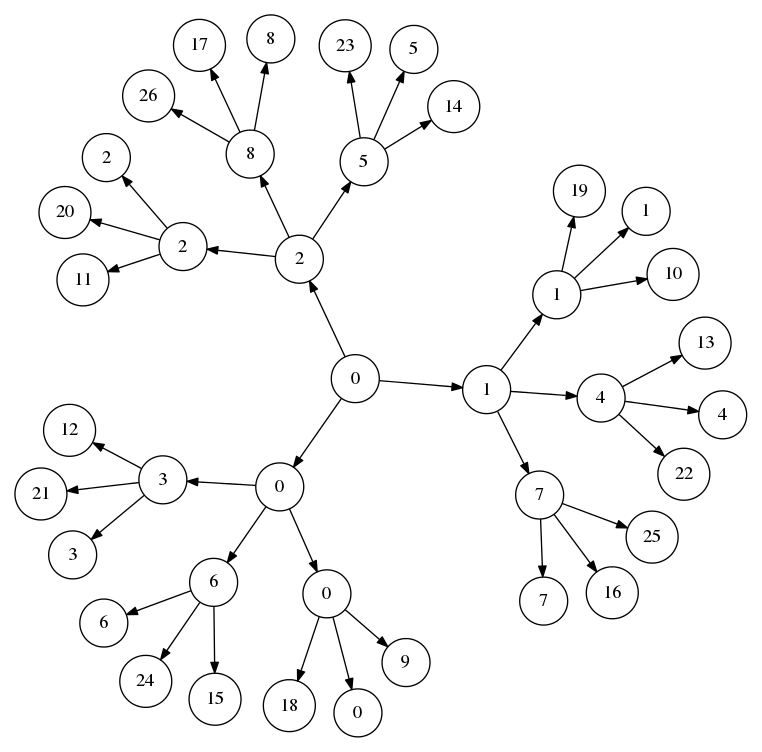
\includegraphics[width=0.85\linewidth]{images/drzewo.png}}
 \captionof{figure}{Rzekomo jest to drzewiasta struktura $\Z_3$.}
\end{Figure}

%%% skompilowane przez neato
% digraph G {
%     nodesep=0.3;
%     ranksep=0.2;
%     margin=0.1;
%     node [shape=circle];
%     edge [arrowsize=0.8];
% 	ae [label="0"]; 
% 	aq [label="0"]; 
% 	ar [label="1"]; 
% 	aw [label="2"]; 
% 	de [label="0"];
% 	dq [label="3"];
% 	dr [label="6"];
% 	dw [label="1"];
% 	ee [label="4"];
% 	eq [label="7"];
% 	er [label="2"];
% 	ew [label="5"];
% 	fe [label="8"];
% 	fq [label="0"];
% 	fr [label="9"];
% 	fw [label="18"];
% 	ge [label="3"];
% 	gq [label="12"];
% 	gr [label="21"];
% 	gw [label="6"];
% 	qe [label="15"];
% 	qq [label="24"];
% 	qr [label="1"];
% 	qw [label="10"];
% 	re [label="19"];
% 	rq [label="4"];
% 	rr [label="13"];
% 	rw [label="22"];
% 	se [label="7"];
% 	sq [label="16"];
% 	sr [label="25"];
% 	sw [label="2"];
% 	te [label="11"];
% 	tq [label="20"];
% 	tr [label="5"];
% 	tw [label="14"];
% 	we [label="23"];
% 	wq [label="8"];
% 	wr [label="17"];
% 	ww [label="26"];
% 	de -> fq;
% 	de -> fr;
% 	de -> fw;
% 	dq -> ge;
% 	dq -> gq;
% 	dq -> gr;
% 	dr -> gw;
% 	dr -> qe;
% 	dr -> qq;
% 	dw -> qr;
% 	dw -> qw;
% 	dw -> re;
% 	ee -> rq;
% 	ee -> rr;
% 	ee -> rw;
% 	eq -> se;
% 	eq -> sq;
% 	eq -> sr;
% 	er -> sw;
% 	er -> te;
% 	er -> tq;
% 	ew -> tr;
% 	ew -> tw;
% 	ew -> we;
% 	fe -> wq;
% 	fe -> wr;
% 	fe -> ww;
%     ae -> aq;
%     ae -> ar;
%     ae -> aw;
%     aq -> de;
%     aq -> dq;
%     aq -> dr;
%     ar -> dw;
%     ar -> ee;
%     ar -> eq;
%     aw -> er;
%     aw -> ew;
%     aw -> fe;
% }

\begin{fakt}
	W niearchimedesowym ciele $\cialo$ każdy punkt kuli (otwartej, domkniętej) jest jej środkiem.
	Jeśli $r > 0$, to kula jest otwarnięta.
	Dwie kule (domknięte, otwarte) są rozłączne lub zawarte jedna w drugiej.
\end{fakt}

\begin{proof}
	Wszystko jest proste, tylko nic nie jest oczywiste.
	\begin{enumx}
		\item Jeśli $y \in \kula(x, r)$, to $\|x-y\| < r$.
		Biorąc dowolny $z$, że $\|z-x\| < r$, dostajemy $\|z-y\| < r$ (niearchimedesowo), zatem $\kula(x,r) \subset \kula(y,r)$.
		Podobnie w drugą stronę.
		\item Każda otwarta kula jest otwartym zbiorem.
		Weźmy $y$ z brzegu $\kula(x,R)$, do tego $r \le R$.
		Wtedy pewien $z$ jest w $\kula(x,R) \cap \kula(y,r)$ (przekrój jest niepusty).
		To oznacza, że $\|z-x\| < R$ oraz $\|z - y\| < r \le R$, więc $\|x-y\| \le R$ i $y \in \kula(x,R)$.
		\item Weźmy nierozłączne $\kula(x,r)$, $\kula(y,R)$, że $r \le R$.
		Wtedy pewien $z$ leży w obydwu kulach.
		Ale $\kula(x,r) = \kula(z,r)$ zawiera się w $\kula(z,R) = \kula(y,R)$. \qedhere
	\end{enumx}
\end{proof}

Efektem ubocznym jest to, że gdy $\cialo = \Q$, zaś $\|\cdot\| = |\cdot|_p$, to domknięte kula $\kula [0,1]$ jest sumą rozłączną otwartych $\kula (i, 1)$ dla $0 \le i < p$.
,,Sfera'' ($\{x \in \cialo : \|x-y\| = r\}$) jest otwarnięta (i \emph{nie jest} brzegiem kuli).

Nietrywialne otwarte kule niczym nie różnią się od swoich domkniętych koleżanek.
To pokazuje, do jak wielu fałszywych wniosków można dojść myśląc o przestrzeniach metrycznych jak o $\R^n$.

Cassels nazywa nasze normy waluacjami, a przy tym upiera się przy innej nierówności:
$\|x+y\| \le C \max \{\|x\|, \|y\|\}$.
Na stałą $C = 2$ można sobie pozwolić zawsze (zmieniając normę, ale nie topologię) i dostać nierówność trójkąta, na $C= 1$ (ultra) już niekoniecznie.